% easychair.tex,v 3.5 2017/03/15

\documentclass{easychair}

\usepackage{doc}

\newcommand{\easychair}{\textsf{easychair}}
\newcommand{\miktex}{MiK{\TeX}}
\newcommand{\texniccenter}{{\TeX}nicCenter}
\newcommand{\makefile}{\texttt{Makefile}}
\newcommand{\latexeditor}{LEd}

\usepackage{eurosym}
\usepackage{graphicx}

\title{Cybersecurity Impacts of the Covid-19 Pandemic in Italy}

\author{
  Marco R.A.\ Bozzetti\inst{1,2,3}
  \and
  Luca Olivieri\inst{4}
  \and
  Fausto Spoto\inst{4}
}

% Institutes for affiliations are also joined by \and,
\institute{
  Associazione Italiana Professionisti della Sicurezza Informatica (AIPSI), Milano, Italy
\and
  Italian Information System Security Association International (ISSA)
\and
Digital Attacks Observatory (OAD) Team, Italy\\
\email{m.bozzetti@aipsi.org}
\and
   University of Verona, Verona, Italy\\
   \email{\{luca.olivieri,fausto.spoto\}@univr.it}\\
 }

\authorrunning{M.\ Bozzetti, L.\ Olivieri, F.\ Spoto}

\titlerunning{Cybersecurity impacts at the beginning of Covid-19 pandemic in Italy}

\begin{document}

\maketitle

\begin{abstract}
  The Covid-19 pandemic has pushed companies to the extensive
  use of digital services, to implement home working and provide
  online services to people in lockdown. As a consequence, it is interesting
  to study how this has affected the number, kind and distribution of cybersecurity
  attacks. This paper gives an empirical evaluation of the cybersecurity attacks
  at the beginning of the Covid-19 pandemic in Italy, based on data collected from
  the questionnaires of the annual Digital Attacks Observatory. It shows that the overall
  number of attacks has not increased, but attacks have affected smaller companies
  than before. This can be explained with the fact that the Italian
  industrial scenario is mostly populated by small and medium enterprises,
  that have been obliged to a quick reconvertion of their IT systems and typically
  lack the necessary cybersecurity culture.

  \mbox{}\\
  \textbf{Keywords:} cyberattack, cybersecurity, Covid-19, SME.
\end{abstract}

\section{Introduction}

The Covid-19 pandemic and consequent lockdowns have obliged
companies to face new challenges such as smart working, remote work and digitalization,
accelerating all previous efforts in that direction.
As reported by Gartner~\cite{Goasduff20}, most organizations were already moving
their digital agenda forward at a steady pace, but the Covid-19 pandemic required
a significant leap in the 
development of digital products and services, with the goal of
maintaining and fostering customer engagement.
However, digitalization has generated many cybersecurity 
issues and the intensification of cyberattacks all around the world~\cite{HKICS20,PA21}.
In this scenario, Italy is an interesting case study since it is home
of mostly small to medium enterprises (SMEs), active in different sectors,
and can consequently highlight cybersecurity aspects that are different from those
faced by larger companies of greater influence. This paper presents the status of the
Italian scenario, to understand how cyberattacks and cybersecurity have fared
during the ongoing COVID-19 pandemic.
Section~\ref{sec:DigitalAttacksObservatory} presents the \textit{Digital Attacks Observatory},
a survey that we have used to collect relevant information about cybersecurity and 
Italian organizations.
Sections~\ref{sec:DataDiscussion} and~\ref{sec:TypeAttacks} report
a detailed discussion of the collected data and observed trends.
Finally, Section~\ref{sec:Conclusion} concludes by underlying the importance of
a cybersecurity culture focused on the Italian reality.

\section{Digital Attacks Observatory}\label{sec:DigitalAttacksObservatory}

The \textit{Digital Attacks Observatory} (OAD)~\cite{oadweb} is the only independent online survey in Italy about intentional digital attacks on IT systems of companies and public
bodies. It is implemented in collaboration with the Italian postal and telecommunications police.
The last OAD 2020 was the twelfth year of consecutive surveys on cyberattacks in Italy.
The OAD survey is not directed at a predefined set of respondents, but allows potential interested
parties to have full and free access to an online questionnaire, in a totally anonymous way. 
Thanks to the number of responses collected and their balanced distribution between companies and public bodies of different size and belonging to different economic
sectors, we can provide a specific picture of the cyberattacks in Italy.

\subsection{The Questionnaires}

About half of the OAD questionnaires refer to the occurred
cyberattack typologies and their main characteristics.
The other half refers to the technical and organizational security measures implemented
on the IT systems of the respondents. 
Therefeore, OAD allows one to match the cyberattacks to the cyber-measures in each production
IT system considered. 
In fact, OAD provides a qualitative macro-evaluation of the implemented measures
(within the specific context of the company), in order to motivate the anonymous respondents
to complete the questionnaires.
In particular, the security measures considered in the 2020 questionnaire were subdivided
in \emph{technical}, \emph{organizational}, \emph{managerial} and \emph{governamental}, as follow:

\begin{enumerate}
\small
	\item \emph{Technical measures}
	\begin{itemize}
		\item Overall architecture of the digital security measures, integrated with the entire IT system architecture
		\item Physical countermeasures
		\item Identification, Authentication, and Authorization (IAA) measures
		\item Cybersecurity measures at local and geographical network level
		\item Measures for logical protection of each single Information and Communication Technology (ICT) system
		\item Application and software protection
		\item Data protection
	\end{itemize}
	\item \emph{Organizational measures}
	\begin{itemize}
		\item Organizational structure, roles, skills, certifications
		\item Organizational policies and procedures
		\item Contracts, agreements and digital security clauses with third parties
		\item Awareness and culture of digital security at all levels
		\item Auditing
	\end{itemize}
	\item \emph{Managerial and governamental measures}
	\begin{itemize}
		\item Digital security control, monitoring and management systems
		\item Disaster Recovery (DR) plan.
	\end{itemize}
\end{enumerate}

\subsection{Overview from 2019 to 1Q-2020}

The OAD 2020 survey
\footnote{The report is written in Italian,
  only the Executive Summary is in English: 186 A4 pages, 148 images and graphics, 11 Chapters
  (147 A4 pages) and 9 Attachments (39 A4 pages).}~\cite{oad20}
took place during the
Covid-19 pandemic and covered the entire 2019 and the first quarter 
of 2020, when the pandemic exploded in Italy. The comparison of data from 2019 to that
from the first quarter of 2020, provided by the same set of respondents,
has statistical relevance and provides a 
clear indication of the Covid-19 pandemic on the intentional cyberattacks in Italy.
This pandemic has triggered a wide range of cyberattacks, mainly 
caused by the sudden, and partly unexpected, passage to working from home
and to a strong use of every type of IT service on the Internet, as a consequence
of the mobility lockdowns imposed by the Italian authorities. The resulting respondents pool
covers all the production sectors, including public administration,
even if the majority of the respondents companies belong to the ICT sector (30.8\%).
The 2020 pool is well balanced for the size of the organizations, in terms
of employees, between those below 250 and the largest ones. It must be taken into account,
as reported by ISTAT~\cite{istat21}, that 99.91\%
of enterprises in Italy are SMEs, with up to 250 employees, and 95\% have fewer than ten employees.
The OAD 2020 survey is therefore able to consider small and 
tiny organizations, that are the vast majority in Italy, and that usually
are not considered in other cybersecurity surveys: 57.5\% of the OAD 2020 respondents
belong to structures with less than 250 employees and, of these, 22.1\% have fewer than ten
employees. 

\section{Discussion}\label{sec:DataDiscussion}

\begin{figure}
	\centering
		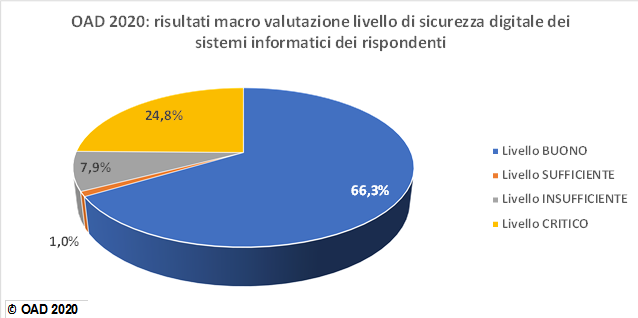
\includegraphics[width=1\textwidth]{pictures/fig1.png}
		\caption{Extract of the OAD 2020~\cite{oad20} on the macro-evaluation
                  of the security level in the IT systems in Italy.
                  The chart shows that more than two thirds of the respondents
                  judge the level of cybersecurity of their IT systems as good.}
		\label{fig:1}
\end{figure}

The data collected in the OAD 2020 show, in general, that the respondents have, for the most part,
a good perception of the cybersecurity of their IT systems (Fig.~\ref{fig:1}).
This information can be explained from the fact that:
 
\begin{itemize}
\item About 30\% of respondents are in the ICT sector, therefore their IT systems
  are managed with some cybersecurity literacy and can properly react to cyberattacks, preventing 
  them or minimizing their effects.

\item In general, cybercriminals do not waste time and resources to attack small businesses,
  where they can only obtain a marginal profit and still
  take the risk of being caught by the police.  As confirmed by the trends shown
  in Fig.~\ref{fig:3}, attackers target the larger companies most,
  because the illegal gain is more interesting in that case.
\end{itemize}

\begin{figure}
  \centering
  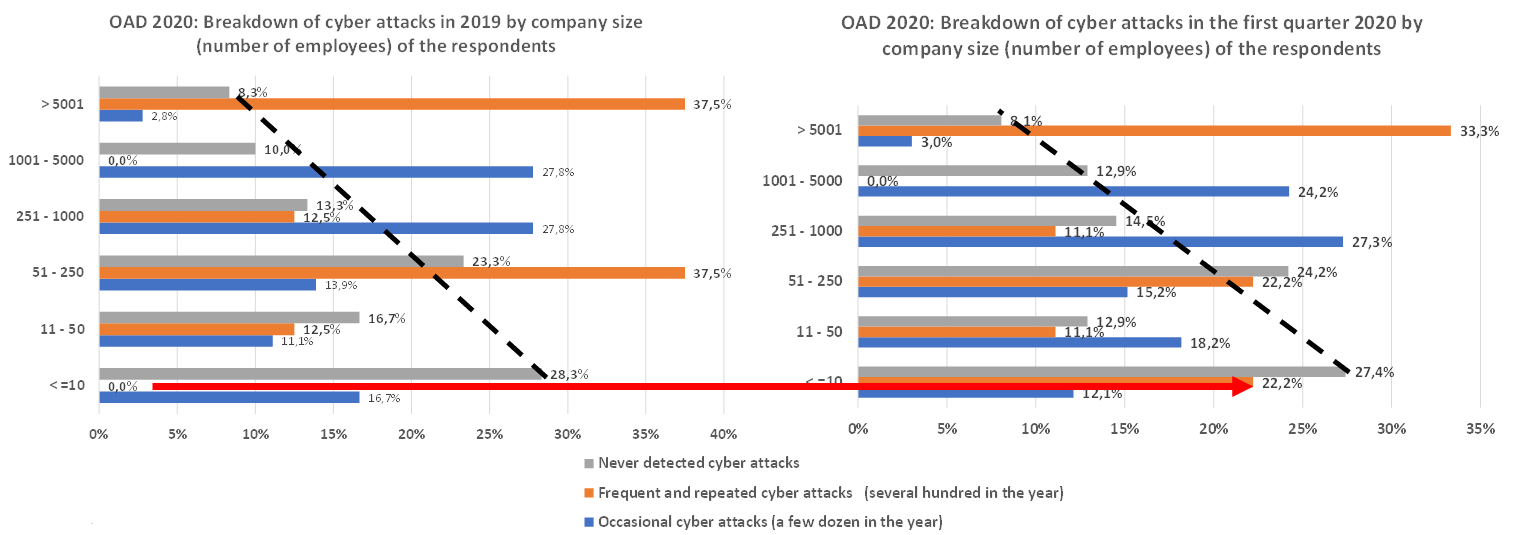
\includegraphics[width=1\textwidth]{pictures/fig3.png}
  \caption{Comparison between cyberattacks occurred in 2019 and in the first quarter of 2020,
    wrt.\ to the organization dimension~\cite{oad20}. The dotted line links
    the unreported attacks and shows that they decrease while moving from tiny to big organizations,
    in terms of employees.}
  \label{fig:3}
\end{figure}


\begin{figure}
  \centering
  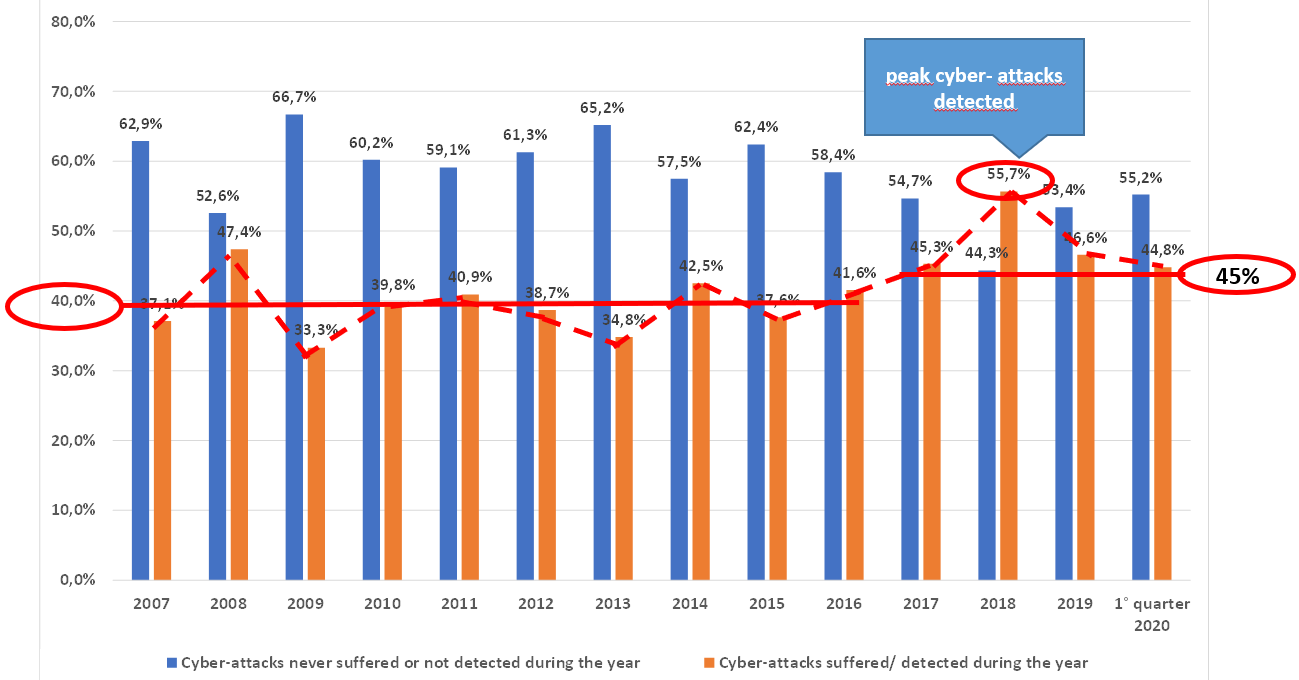
\includegraphics[width=1\textwidth]{pictures/fig2.png}
  \caption{Trend of the reported attacks from the beginning of the OAD survey
    in 2008~\cite{oad20}. This comparison is only valid as a trend and not as a statistical
    measure, since the respondents are different from year to year. The dotted red line shows
    successive waves: after a relative pick of attacks, companies react and strengthen
    their cybersecurity measures, so that, the following year, the trend dicreases.}
  \label{fig:2}
\end{figure}

The chart in Fig.~\ref{fig:2} analyzes the trend of cyberattaks.
The figure shows that, from 2007 to 2015, in average, about 40\% of the respondents
reported cyberattacks (leftmost full red line). Since 2015, the trend increased to 45\%
of the respondents (rightmost full red line). 
In 2018, OAD reached the pick of reported attacks and, for the first time, the percent of
reported attacks became larger than that percent of companies that did not report any attack.
After the pick 
in 2018, year 2019 has a lower figure and the same occurs in the first quarter 2020.
The trend for full 2020 will be discovered with the currently ongoing OAD survey.
This view, over several years, does not show significant changes, not even inside
the pandemic period, but shows only a slight increase in cyberattacks 
in the recent years, not necessarily attributable to the pandemic crisis.

As already highlighted above, the comparison between the whole 2019 and the first quarter 2020
in Fig.~\ref{fig:3} maintains the same logical trend. The only meaningful difference
is in the number of attacks reported by the smallest
organizations (up to ten employees): they were 0\% in 2019 and grwo to
22,2\% at the beginning of 2020 (see the red arrow in Fig.~\ref{fig:3}).
Such a strong increase follows from the extensive use of e-banking and 
e-commerce services, with the related cyberattacks.

The impact of the pandemic on the cybersecurity in Italy is also highlighted by the data
provided by the postal and communication police, that shows the situation for the
critical infrastructures (Table~\ref{tab:table1}), for the financial cyber-crimes
(Table~\ref{tab:table2}) and for the cyber-terrorism (Table~\ref{tab:table3}). 
Fraudulent transactions in 2019 were blocked for a total value of \euro 21.3 million and \euro 18 million were recovered; in the first quarter of 
2020, fraudulent transactions for \euro 20.2 million were blocked,
practically reaching in four months the amount
blocked in the full twelve months of 2019, and \euro 8 million have been
recovered. This is an indication of the increase in attacks on financial transactions
and services due to the very large use of these online services, caused by the mobility reduction
measures consequent of the Covid-19 pandemic.

\begin{table}[h]
  \begin{center}
  \resizebox{1\textwidth}{!}{
	\begin{tabular}{|r|r|r|r|r|r|}									
		\hline
		\textbf{Critical structure protection}	&	1 Jan - 30 Apr	&	1 Jan - 31 Dec	&	1 Jan - 31 Dec &	1 Jan - 31 Dec &	1 Jan - 31 Dec\\
                	&	2020	&	2019	&	2018 &	2017 &	2016\\
		\hline									
		Relevant attacks	&	282	&	1.181	&	459	&	1.032 & 844	\\
		Issued alerts	&	24.824	&	82.484	&	80.777	&	31.524 & 6.721	\\
		Initiated investigations 	&	34	&	155	&	74	&	72 & 70	\\
		People arrested	&	0	&	3	&	1	&	3	& 3\\
		People reported	&	0	&	117	&	14	&	1.316 &	1.226	\\
		Perquisitions	&	n.d.	&	n.d.	&	n.d.	&	73	& 58 \\
		\hline	
		Initiated investigations	&	12,05\%	&	13,12\%	&	16,12\%	&	6,98\%	& 8,29\% \\
		\hline	
		People arrested out ofreported &	0\%	&	2,5\%	&	7,14\%	&	0,23\%	&	0,24\%\\						
		\hline	
	\end{tabular}
	}
    \end{center}
	
	\caption{Data of critical structure protection collected by Italian postal and communication police~\cite{oad20}.}									
	\label{tab:table1}									
\end{table}	

\begin{table}[h]
  \begin{center}
  \resizebox{1\textwidth}{!}{
	\begin{tabular}{|r|r|r|r|r|r|}									
		\hline									
		\textbf{Financial Cyber Crime}	&	1 Jan - 30 Apr	&	1 Jan - 31 Dec	&	1 Jan - 31 Dec &	1 Jan - 31 Dec &	1 Jan - 31 Dec\\
                	&	2020	&	2019	&	2018 &	2017 &	2016\\
		\hline									
		Blocked fraudulent transactions	&	\textbf{\euro 20.200.000,00}	&	\textbf{\euro 21.333.990,00}	&	\euro 38.400.000,00	& \euro 20.839.576,00 & \euro 16.050.812,50 	\\
		Recovered amounts 	&	\euro 8.700.000,00	&	\euro 18.000.000,00	&	\euro 9.000.000,00	&	\euro 862.000,00 & n.a.	\\
		People arrested	&	n.a.	&	n.a.	&	n.a.	&	25	& 25\\
		People reported	&	n.a.	&	n.a.	&	n.a.	&	2.851 & 3.772	\\
		\hline	
		Recovered amounts out of fraud	&	12,05\%	&	13,12\%	&	16,12\%	&	6,98\%	& 8,29\% \\
		\hline	
	\end{tabular}
	}
    \end{center}
	\caption{Data of critical structure protection collected by Italian postal and communication police~\cite{oad20}.}									
	\label{tab:table2}									
\end{table}	

\begin{table}[h]
  \begin{center}
	\begin{tabular}{|r|r|r|r|}									
		\hline									
		\textbf{Cyber-terrorism}	&	1 Jan - 30 Apr 2020	&	1 Jan - 31 Dec 2019	&	1 Jan - 31 Dec 2018\\
		\hline									
		Monitored web space	&	\euro 11.962	&	\euro 36.377	&	\euro 36.000\\
		Removed contents 	&	n.a.\	&	n.a.\	&	250\\
		\hline	
	\end{tabular}
        \end{center}
	\caption{Data of cyber terrorism collected by Italian Postal and Communications Police~\cite{oad20}}									
	\label{tab:table3}									
\end{table}	

\section{Nature of Cyberattacks}\label{sec:TypeAttacks}

In the pandemic period, between 2019 and the first quarter of 2020, the nature of the attacks and their vectors were quite diversified.
The attacks on IAA that aimed at access control systems are widespread, since they amount to 28.2\% of the total attacks
of 2019 and to 34\% of the total attacks in the first quarter of 2020 (Fig.~\ref{fig:5}).

\begin{figure}
  \centering
  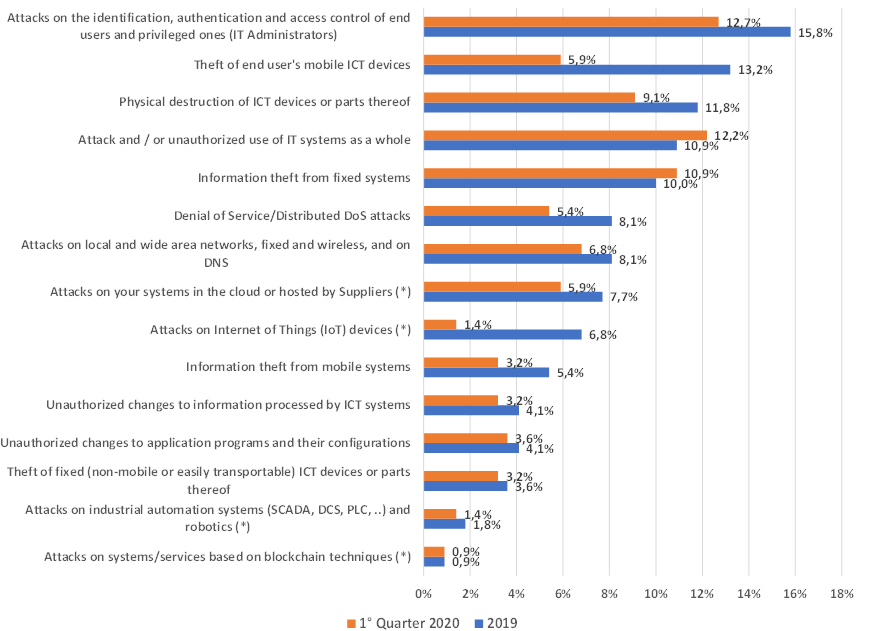
\includegraphics[width=1\textwidth]{pictures/fig5.png}
  \caption{Widespread of the digital attacks on the respondents' computer systems, classified wrt.\ the type of attack, between 2019 and the first quarter of 2020 (multiple answers)~\cite{oad20}.}
  \label{fig:5}
\end{figure}

The other 14 types of attacks follow, decreasing by a few percent points between them, whose characteristics and impacts are detailed in the related 
paragraphs of the OAD 2020 report. Regarding attack vectors and techniques, all the seven attack families considered in the 2020 questionnaire are widely used in the various 
types of attacks, sometime even simultaneously, as shown in Fig.~\ref{fig:6}. The trend in Fig.~\ref{fig:6} is also in line with most European reports, such as
that of the European Network and Information Security Agency (ENISA)~\cite{enisa20}. 
The most widespread one, in the average of the various attacks detected by the respondents, is the use of toolkits (rootkits, meta-exploits, etc.)
for the identification and exploitation of vulnerabilities
on the target system, with 38.8\%, followed by the well-known malicious and unauthorized collection of information (social engineering, phishing, etc.), with 34.6\%,
and the use of malicious code and scripts, with 34.3\%. The other considered techniques decrease, with a few percent points between them. The impacts of the most 
critical attacks are analyzed, for each attack type, as well as their possible motivations and the recovery time required by the most critical ones.
In the 2020 OAD survey, all these attack characteristics vary for each type of attack, and the emerged results are described in the specific paragraphs dedicated to each attack 
type. In the overall, it emerges that:
\begin{itemize}
\item the impacts declared by the respondents are balanced between those irrelevant and/or easily resolvable with a quick recovery and at limited costs, and those very 
critical, that require expensive and long recovery actions and that, in some cases, can cause business and customer losses. These two very different impact cases depend mainly 
on the security measures in place;
\item the motivations of the cyberattacks are mainly economic, such as fraud and blackmailing: the widespread diffusion of ransomware in Italy is a clear 
confirmation of these motivations.
\end{itemize}

\begin{figure}
  \centering
  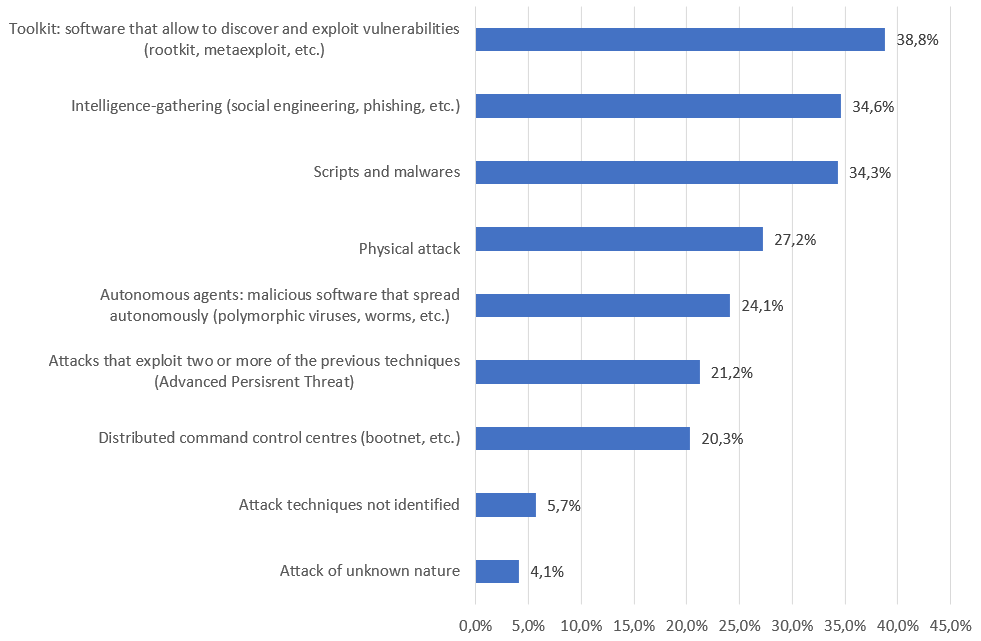
\includegraphics[width=0.90\textwidth]{pictures/fig6.png}
  \caption{Average diffusion (in percent) of the attack techniques detected in the most serious attacks between 2019 and the first quarter of 2020 (multiple answers)~\cite{oad20}.}
  \label{fig:6}
\end{figure}

As pointed out in Fig.~\ref{fig:1}, the IT systems considered in the 2020 survey and their cybersecurity are in the medium to high range and the collected information shows a relevant 
improvement in both technical and organizational measures, in comparison to the previous surveys. Few of the considered Italian IT systems are based on data centers in 
Italy: most of the respondents' companies have medium to small IT systems partly on premise and partly outsourced, with an increasing use of cloud services.
The high number of attacks detected in 2018, and the privacy obligations related to the European
General Data Protection Regulation (GDPR), have certainly contributed to strengthening cybersecurity measures, and a further improvement 
comes from the growing use of cloud services, where high standard security measures are in place, usually. Organizational measures for cybersecurity, historically missing and neglected
in Italy, have improved in terms of defition of roles and separation of duties, of organizational policies and procedures, and of incident management. These measures often are missing
in small organizations, and in general the cybersecurity awareness and competence are low, and mainly concentrated at the top level of the public and private organizations. In Italy, there is 
still a long way to go in terms of cybersecurity continued training and awareness. A formal and bureaucratic approach to the organizational procedures is still prevalent. Once defined,
such procedures often do not find concrete application and misses periodic updates and operational tests. A significant example is the disaster recovery plans, for 
which, typically, the required alternative IT resources are neither forecast nor allocated. Periodic exercises and simulations of the 
possible disasters are not implemented. Cybersecurity management tools have limited diffusion yet, among the 2020 OAD respondents. This is particularly true for
the most advanced ones, based on artificial intelligence.
Although the use of IoT~\cite{JK21}, industrial automation, robotics systems~\cite{SGLMDXHKCZT21} and systems based on blockchain technology~\cite{RMFF21}
are expanding and can contribute to fight the Covid-19 pandemic.
In the OAD 2020 report, one finds only a few respondents involved in such technologies, which also derives from the limited portion
of their economic sector, interested in such systems: the manufacturing sectors, the logistics, the research and 
development centers and labs, the local public administration for territorial control, and so on.
%For these topics, the data that emerged from the survey are considered only as 
%specific cases that contribute to the general values on the cyberattacks, but which cannot be still considered of reference at the Italian level.

\section{Conclusion}\label{sec:Conclusion}

The OAD 2020 survey highlights the presence of cyberattacks of various types in Italy, all technically of an high complexity and sophistication, with a slight increase 
compared to the trend that emerged in the twelve years of the previous OAD surveys, but still below the pick of 2018. Despite the proliferation of cyberattacks
related to the Covid-19 pandemic, in the first four months of 2020 the widespread of attacks is at a level similar to that of 2019. This will be better verified
with the next OAD 2021. The Italian reality, made up of a very large number of small and tiny organizations, does not make our country very attractive to cybercriminals, but cyber-warfare
and massive attacks represent a growing and serious risk, as has already occurred with the widespread of ransomware on computer systems with no or low
measures of cybersecurity. The OAD 2020 shows a clear improvement and strengthening of digital security measures, both technical and organizational, even if the most modern 
prevention, protection and management systems that use artificial intelligence techniques are still in their infancy among the respondents. The defense measures and techniques 
in use fight the increasingly sophisticated and smart evolution of attacks, but often too late. The high density of vulnerabilities 
requires different approaches, aiming at making all IT systems interconnected to the Internet and safe, by default and by design. But we are 
still a long way from this goal. In order to improve the actual fight against continuous attacks and cybercrime, it is currently necessary to increase 
awareness on cybersecurity and skills at all levels. It is also paramount to support an effective collaboration between police bodies at the international level.

\bibliographystyle{plain}
\bibliography{biblio}

\end{document}

